\documentclass[letterpaper]{article}
\usepackage[utf8]{inputenc}
\parskip 7.2pt

\title{Homework 05 Key. PLS206 Fall 2013}
\author{Emilio A. Laca}

\usepackage{Sweave}
\begin{document}
\Sconcordance{concordance:HW05Key.tex:HW05Key.Rnw:%
1 7 1 1 0 12 1 1 2 1 0 2 1 15 0 3 1 3 0 1 2 6 1 1 2 1 0 1 1 19 0 1 1 6 %
0 1 1 14 0 1 1 17 0 1 2 4 1 1 2 4 0 1 3 4 0 1 2 2 1 1 -7 1 11 7 1 1 -15 %
1 19 8 1 1 2 7 0 1 2 10 1 1 2 1 0 2 1 18 0 1 1 4 0 1 2 48 1}


\maketitle

\section{PCA, PCR and PLSR}
Read and use sections 9.2 and 9.3 of Faraway-PRA as a guide.
Use the meatspec data file.

The intensity of radiation in each of 100 frequency bands (V1-V100) was measured for 215 samples of meat using a Near Infrared Transmission (NIT) analyzer. Each sample was also analyzed for fat content using a more expensive and time consuming wet-chemistry method.

Exclude the last 43 observations for adjusting the models.

\begin{Schunk}
\begin{Sinput}
> library(faraway)
> data(meatspec)
> names(meatspec)
\end{Sinput}
\begin{Soutput}
  [1] "V1"   "V2"   "V3"   "V4"   "V5"   "V6"   "V7"   "V8"   "V9"   "V10" 
 [11] "V11"  "V12"  "V13"  "V14"  "V15"  "V16"  "V17"  "V18"  "V19"  "V20" 
 [21] "V21"  "V22"  "V23"  "V24"  "V25"  "V26"  "V27"  "V28"  "V29"  "V30" 
 [31] "V31"  "V32"  "V33"  "V34"  "V35"  "V36"  "V37"  "V38"  "V39"  "V40" 
 [41] "V41"  "V42"  "V43"  "V44"  "V45"  "V46"  "V47"  "V48"  "V49"  "V50" 
 [51] "V51"  "V52"  "V53"  "V54"  "V55"  "V56"  "V57"  "V58"  "V59"  "V60" 
 [61] "V61"  "V62"  "V63"  "V64"  "V65"  "V66"  "V67"  "V68"  "V69"  "V70" 
 [71] "V71"  "V72"  "V73"  "V74"  "V75"  "V76"  "V77"  "V78"  "V79"  "V80" 
 [81] "V81"  "V82"  "V83"  "V84"  "V85"  "V86"  "V87"  "V88"  "V89"  "V90" 
 [91] "V91"  "V92"  "V93"  "V94"  "V95"  "V96"  "V97"  "V98"  "V99"  "V100"
[101] "fat" 
\end{Soutput}
\begin{Sinput}
> train <- meatspec[1:172,]
> validate <- meatspec[173:215,]
> rmse <- function(x,y) sqrt(mean((x-y)^2)) #make a function to calculate the square root of the mean squared error
\end{Sinput}
\end{Schunk}

 We made two separate datasets, "train" is the training set, and "validate" is the validation data. The function rmse facilitates the calculation of the square root of the mean squared prediction error.
\section {PCA}
\subsection {Perform an analysis of principal components of variables V1-V100 based on the correlation matrix. [10]}

Make sure that you do not include "sample" or "fat." Report the eigenvector elements for PC2, V1-V3.

\begin{Schunk}
\begin{Sinput}
> meatpca <- prcomp(meatspec[1:172,-101], scale.=TRUE)
> str(meatpca)
\end{Sinput}
\begin{Soutput}
List of 5
 $ sdev    : num [1:100] 9.925 1.044 0.536 0.331 0.079 ...
 $ rotation: num [1:100, 1:100] 0.0996 0.0996 0.0996 0.0996 0.0996 ...
  ..- attr(*, "dimnames")=List of 2
  .. ..$ : chr [1:100] "V1" "V2" "V3" "V4" ...
  .. ..$ : chr [1:100] "PC1" "PC2" "PC3" "PC4" ...
 $ center  : Named num [1:100] 2.81 2.82 2.82 2.82 2.82 ...
  ..- attr(*, "names")= chr [1:100] "V1" "V2" "V3" "V4" ...
 $ scale   : Named num [1:100] 0.402 0.405 0.407 0.41 0.412 ...
  ..- attr(*, "names")= chr [1:100] "V1" "V2" "V3" "V4" ...
 $ x       : num [1:172, 1:100] -4.471 0.899 -7.329 -1.936 0.877 ...
  ..- attr(*, "dimnames")=List of 2
  .. ..$ : chr [1:172] "1" "2" "3" "4" ...
  .. ..$ : chr [1:100] "PC1" "PC2" "PC3" "PC4" ...
 - attr(*, "class")= chr "prcomp"
\end{Soutput}
\begin{Sinput}
> meatpca$rotation[1:3,2]
\end{Sinput}
\begin{Soutput}
       V1        V2        V3 
0.1296777 0.1306013 0.1314935 
\end{Soutput}
\begin{Sinput}
> rownames(meatpca$rotation)
\end{Sinput}
\begin{Soutput}
  [1] "V1"   "V2"   "V3"   "V4"   "V5"   "V6"   "V7"   "V8"   "V9"   "V10" 
 [11] "V11"  "V12"  "V13"  "V14"  "V15"  "V16"  "V17"  "V18"  "V19"  "V20" 
 [21] "V21"  "V22"  "V23"  "V24"  "V25"  "V26"  "V27"  "V28"  "V29"  "V30" 
 [31] "V31"  "V32"  "V33"  "V34"  "V35"  "V36"  "V37"  "V38"  "V39"  "V40" 
 [41] "V41"  "V42"  "V43"  "V44"  "V45"  "V46"  "V47"  "V48"  "V49"  "V50" 
 [51] "V51"  "V52"  "V53"  "V54"  "V55"  "V56"  "V57"  "V58"  "V59"  "V60" 
 [61] "V61"  "V62"  "V63"  "V64"  "V65"  "V66"  "V67"  "V68"  "V69"  "V70" 
 [71] "V71"  "V72"  "V73"  "V74"  "V75"  "V76"  "V77"  "V78"  "V79"  "V80" 
 [81] "V81"  "V82"  "V83"  "V84"  "V85"  "V86"  "V87"  "V88"  "V89"  "V90" 
 [91] "V91"  "V92"  "V93"  "V94"  "V95"  "V96"  "V97"  "V98"  "V99"  "V100"
\end{Soutput}
\begin{Sinput}
> colnames(meatpca$rotation)
\end{Sinput}
\begin{Soutput}
  [1] "PC1"   "PC2"   "PC3"   "PC4"   "PC5"   "PC6"   "PC7"   "PC8"   "PC9"  
 [10] "PC10"  "PC11"  "PC12"  "PC13"  "PC14"  "PC15"  "PC16"  "PC17"  "PC18" 
 [19] "PC19"  "PC20"  "PC21"  "PC22"  "PC23"  "PC24"  "PC25"  "PC26"  "PC27" 
 [28] "PC28"  "PC29"  "PC30"  "PC31"  "PC32"  "PC33"  "PC34"  "PC35"  "PC36" 
 [37] "PC37"  "PC38"  "PC39"  "PC40"  "PC41"  "PC42"  "PC43"  "PC44"  "PC45" 
 [46] "PC46"  "PC47"  "PC48"  "PC49"  "PC50"  "PC51"  "PC52"  "PC53"  "PC54" 
 [55] "PC55"  "PC56"  "PC57"  "PC58"  "PC59"  "PC60"  "PC61"  "PC62"  "PC63" 
 [64] "PC64"  "PC65"  "PC66"  "PC67"  "PC68"  "PC69"  "PC70"  "PC71"  "PC72" 
 [73] "PC73"  "PC74"  "PC75"  "PC76"  "PC77"  "PC78"  "PC79"  "PC80"  "PC81" 
 [82] "PC82"  "PC83"  "PC84"  "PC85"  "PC86"  "PC87"  "PC88"  "PC89"  "PC90" 
 [91] "PC91"  "PC92"  "PC93"  "PC94"  "PC95"  "PC96"  "PC97"  "PC98"  "PC99" 
[100] "PC100"
\end{Soutput}
\end{Schunk}

The matrix whose columns are the eigenvectors that are used to calculate the PC scores is the "rotation" element in the prcomp object that contains all results from the PCA. The matrix columns are named with the PC name, and the rows have the variable names.

\subsection {Make a Scree and a loading plot and report both. [10]}

\begin{Schunk}
\begin{Sinput}
> biplot(meatpca) # Display biplot
\end{Sinput}
\end{Schunk}
\begin{Schunk}
\begin{Sinput}
> plot(meatpca, main="") #Display scree plot
\end{Sinput}
\end{Schunk}

\begin{figure}
\begin{center}
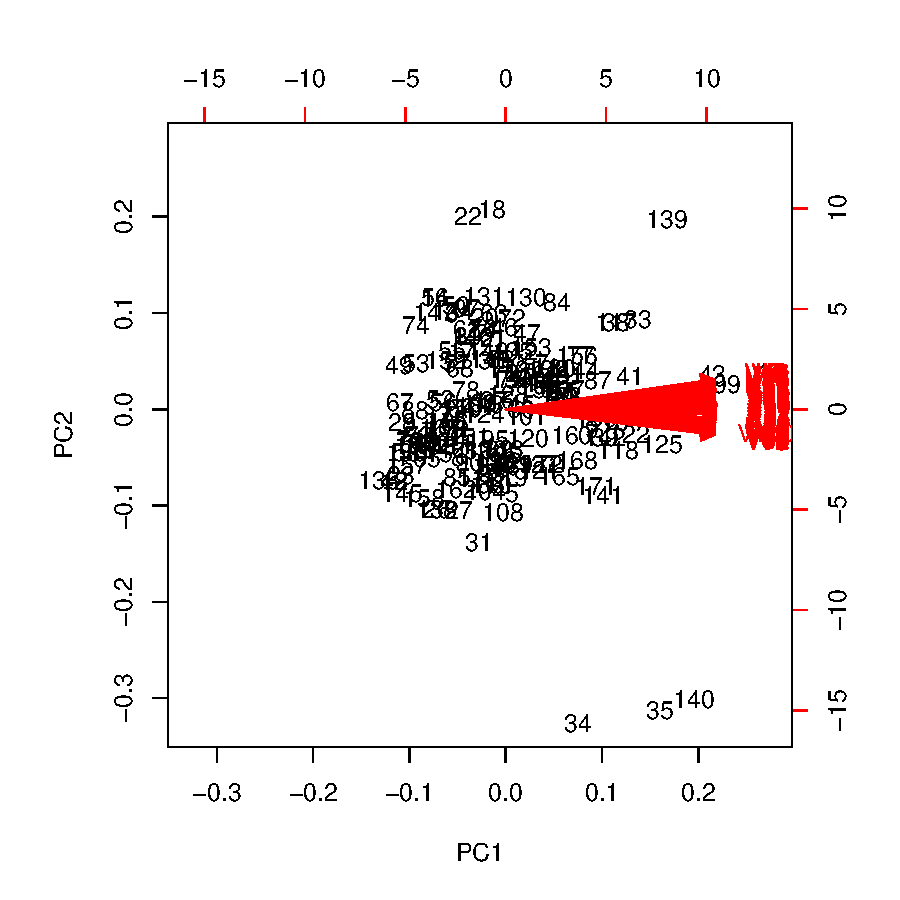
\includegraphics{HW05Key-figbiplot}
\end{center}
\caption{Biplot showing the observations and the arrows constructed with the loadings or correlations between each original variable and the first two PC's.}
\label{fig:qq}
\end{figure}


\begin{figure}
\begin{center}
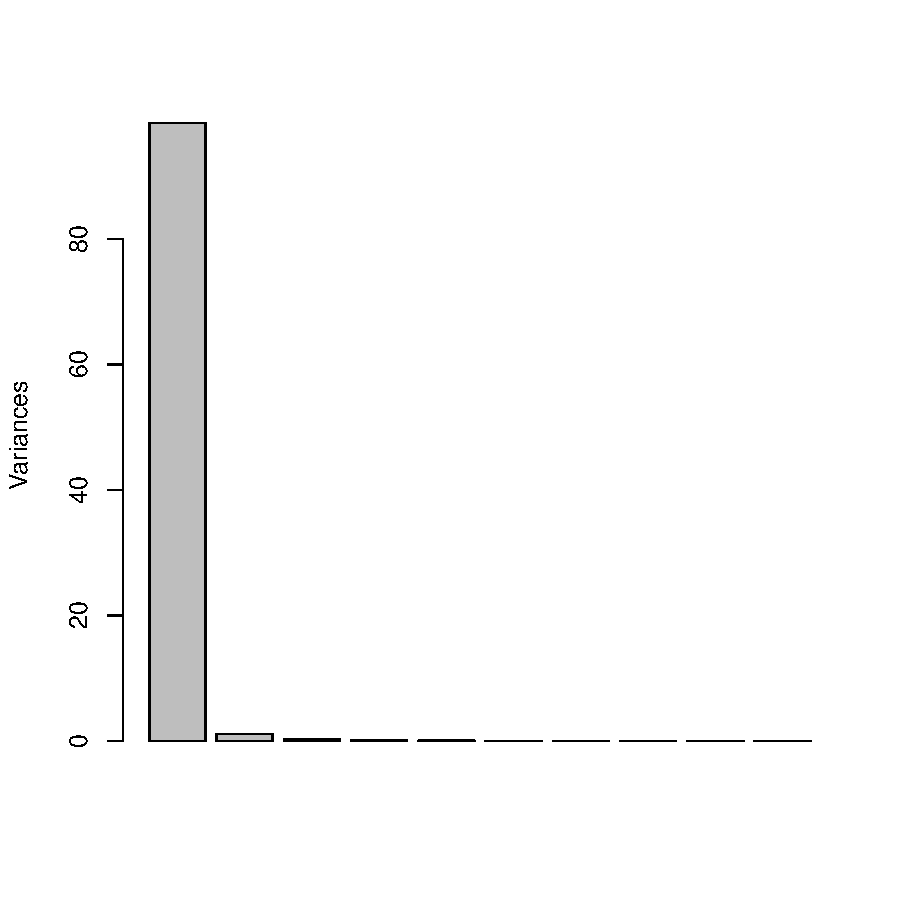
\includegraphics{HW05Key-figscreeplot}
\end{center}
\caption{Scree plot shows the eigenvalues or variances of the principal components in order. In this specific case, the scree plot does not have much value, because we are not trying to describe the structure of the data.}
\label{fig:qq}
\end{figure}

\subsection{What is the loading of V3 on PC2? [10]}

Loadings are the correlations between each variable and each PC. They are also the values used to plot the arrows representing variables in the biplot. Variables with arrows that are long (length close to 1, say, greater than 0.9) are well represented in the subspace or plane formed by the PC's plotted (the default is PC1 and PC2).

\begin{Schunk}
\begin{Sinput}
> cor(meatpca$x[,2],train[,3])
\end{Sinput}
\begin{Soutput}
[1] 0.1372274
\end{Soutput}
\end{Schunk}

\subsection {If your goal were to summarize the information with fewer dimensions, how many PC's would you retain or discuss? Report the number of PC's you retain and the name of the method you used. [10]}

The scree plot shows the eigenvalues in order. This plot can be used to look for breakpoints or "elbows" to select the number of PC's to be retained when using PCA for detecting and describing the structure of a data matrix. In the case of the meat samples, the first PC accounts for most of the variance. This PC1 essentially measures the total amount of light that is transmitted through the sample. Since we are not interested in studying the structure of the data matrix but in making good estimations of the fat content of the sample, no further interpretation would be needed.

The number of PC's to be retained can be selected by inspecting the scree plot, by looking at the cumulative variance accounted for the PC's, by keeping those PC's that are greater than the average (1 if using the correlation matrix), or by keeping those PC's whose eigenvalues are significantly greater than 1. Eigenvalues near 1 indicate that there is not correlation  in the data.

\subsection {Use principal components regression to develop a good model to predict fat content based on the NIT measurement of samples. [30]}

Consider up to 40 PC's. Select the model with the lowest MSPR for the validation data held out. Report the model selected and the MSPR.

\begin{Schunk}
\begin{Sinput}
> library(pls)
> pcrmod <- pcr(fat ~ ., data=train, validation="CV",ncomp=40)
> RMSEP(pcrmod, newdata=validate)
\end{Sinput}
\begin{Soutput}
(Intercept)      1 comps      2 comps      3 comps      4 comps      5 comps  
     12.971       12.503       12.321        9.652        4.534        3.534  
    6 comps      7 comps      8 comps      9 comps     10 comps     11 comps  
      2.821        2.861        2.815        2.790        2.779        2.603  
   12 comps     13 comps     14 comps     15 comps     16 comps     17 comps  
      2.610        2.618        2.753        2.526        2.261        2.079  
   18 comps     19 comps     20 comps     21 comps     22 comps     23 comps  
      2.127        2.293        2.282        2.215        2.162        2.181  
   24 comps     25 comps     26 comps     27 comps     28 comps     29 comps  
      2.146        2.090        1.862        1.855        2.006        1.975  
   30 comps     31 comps     32 comps     33 comps     34 comps     35 comps  
      1.931        1.885        2.065        2.371        2.428        2.444  
   36 comps     37 comps     38 comps     39 comps     40 comps  
      2.418        2.163        2.495        2.578        2.951  
\end{Soutput}
\begin{Sinput}
> validationplot(pcrmod, newdata=validate)
\end{Sinput}
\end{Schunk}
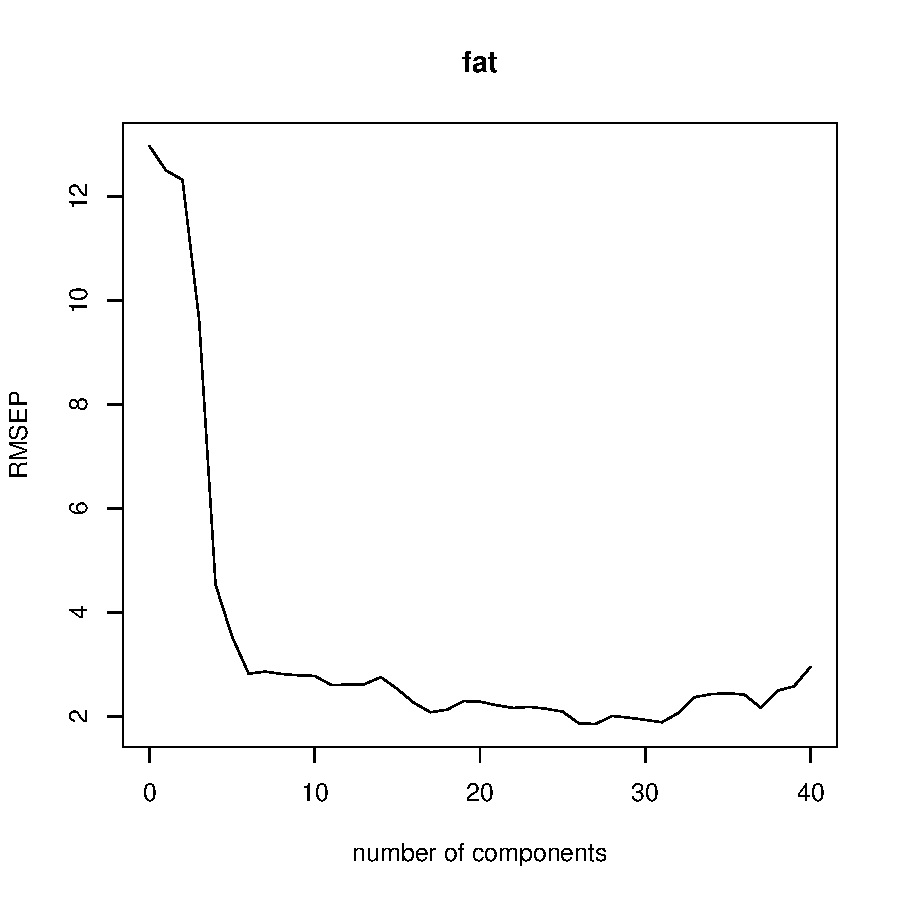
\includegraphics{HW05Key-pcr}

Notice how the RMSEP declines to a minimum of 1.885 with 27 components and then it starts increasing again. The increase is due to overfitting of the model. The model becomes better to predict the training sample, but worse at predicting the validation data.

\subsection {Partial least squares regression. [30]}

Follow the instructions in Faraway-PRA and perform a partial least squares regression of fat on the light transmission data. What does the function sweep() do?

Sweep out Array Summaries

Description

Return an array obtained from an input array by sweeping out a summary statistic.

Usage

sweep(x, MARGIN, STATS, FUN = "-", check.margin = TRUE, ...)
Arguments

x  
an array.

MARGIN	
a vector of indices giving the extent(s) of x which correspond to STATS.

STATS	
the summary statistic which is to be swept out.

FUN	
the function to be used to carry out the sweep.

check.margin	
logical. If TRUE (the default), warn if the length or dimensions of STATS do not match the specified dimensions of x. Set to FALSE for a small speed gain when you know that dimensions match.

...	
optional arguments to FUN.

Details

FUN is found by a call to match.fun. As in the default, binary operators can be supplied if quoted or backquoted.

FUN should be a function of two arguments: it will be called with arguments x and an array of the same dimensions generated from STATS by aperm.

The consistency check among STATS, MARGIN and x is stricter if STATS is an array than if it is a vector. In the vector case, some kinds of recycling are allowed without a warning. Use sweep(x, MARGIN, as.array(STATS)) if STATS is a vector and you want to be warned if any recycling occurs.

Value

An array with the same shape as x, but with the summary statistics swept out.

\end{document}
